\chapter{Inverses and Transformations}


\section{Inverses}

Put on your socks, then your shoes. To undo that, you take off your shoes,
then your socks. Undoing is a big idea in math, and for functions it is
called the inverse.

If a function $f$ is a machine that turns $x$ into $y$, its
\index{inverse function}\newterm{inverse}, written $f^{-1}$, is the machine
that turns $y$ back into $x$.

For example, let $f(x) = 5x + 1$. The rule is ``multiply by 5, then add 1.''
To undo it, subtract 1, then divide by 5: $f^{-1}(x) = (x - 1)/5$. Spot
check: $f(3) = 16$ and $f^{-1}(16) = 3$.

Does $f(x) = x^3$ have an inverse? Yes: $f^{-1}(x) = \sqrt[3]{x}$. Here is
the function (solid) and its inverse (dashed):

\begin{figure}[H]
  \centering
  \begin{tikzpicture}
    \begin{axis}[
        xmin=-3.5,xmax=3.5,
        ymin=-3.5,ymax=3.5,
        ytick={-3,-2,-1,0,1,2,3},
        axis x line=middle,
        axis y line=middle,
        axis line style=<->,
        xlabel={$x$},
        ylabel={$y$},
      ]
      \addplot[thick,no marks,sdkblue] expression[domain=-3:3,samples=100]{x^3};
      \addplot[thick,no marks,sdkblue,dashed] expression[domain=0:3,samples=100]{x^(1/3)};
      \addplot[thick,no marks,sdkblue,dashed] expression[domain=-3:0,samples=100]{-1 * (-1 * x)^(1/3)};
    \end{axis}
  \end{tikzpicture}
  \caption{The function $f(x) = x^3$ and its inverse.}
  \label{fig:inv1}
\end{figure}


The inverse is the same curve with the axes swapped: every point $(a, b)$
on $f$ becomes $(b, a)$ on $f^{-1}$. Swapping coordinates
\emph{reflects}\index{reflections} the graph across the line $y=x$.

That gives a recipe for finding an inverse: swap $x$ and $y$, then solve
for $y$.

\textbf{Worked example.} Find the inverse of $f(x) = 2x + 1$.

\textbf{Solution.} Write $y = 2x + 1$ and swap: $x = 2y + 1$. Solve for
$y$: $y = \frac{x - 1}{2}$. So $f^{-1}(x) = \frac{x - 1}{2}$. Check:
$f(f^{-1}(x)) = 2\left(\frac{x-1}{2}\right) + 1 = x$. The inverse undoes
the function, just as it should.

Not every function has an inverse. Take $f(x) = x^2$: $f(2) = f(-2) = 4$.
What would $f^{-1}(4)$ be, 2 or $-2$? There is no way to choose. This gives
the \newterm{horizontal line test}: if any horizontal line hits a function's
graph more than once, the function has no inverse. A function that passes
is \index{one-to-one function}\newterm{one-to-one}: each output comes from
exactly one input.
\index{horizontal line test}
\begin{figure}[H]
  \centering
  \begin{tikzpicture}
    \begin{axis}[
        xmin=-3.5,xmax=3.5,
        ymin=-1, ymax=6,
        ytick={-1,0,1,2,3,4,5,6},
        axis x line=middle,
        axis y line=middle,
        axis line style=<->,
        xlabel={$x$},
        ylabel={$y$},
      ]
      \addplot[thick,no marks,sdkblue] expression[domain=-3:3,samples=100]{x^2};
      \addplot [thick, dashed] coordinates {(-3,4)(3,4)};
    \end{axis}
  \end{tikzpicture}
  \caption{The horizontal line test run on $f(x)=x^2$.}
  \label{fig:hlt_func}
\end{figure}


Sometimes you can rescue an inverse by trimming the domain. If we keep only
the nonnegative inputs, $f(x) = x^2 - 5$ passes the horizontal line test,
and its inverse is $f^{-1}(x) = \sqrt{x + 5}$.

What is the domain of $f^{-1}$? Run every input in the domain of $f$
through the machine and collect what comes out. That set is the
\textit{image}, or \textit{range}\index{range}, of $f$.

The range of $f(x) = x^2 - 5$ is the set of all real numbers greater than
or equal to $-5$. We write this:

\begin{equation*}
  \{ x \in {\rm I\!R} | x \geq -5 \}
\end{equation*}

Now we can say: \textbf{The range (or image) of the function is the domain
  of the inverse function.}

The swap goes both ways: the domain of $f$ is the range of $f^{-1}$. In our
example, you can feed any number greater than or equal to $-5$ into
$f^{-1}$.

\begin{figure}[H]
  \centering
  \begin{tikzpicture}
    \begin{axis}[
        xmin=-5.5,xmax=7.5,
        ymin=-6, ymax=5,
        xtick={-3, 2},
        ytick={-5, 1},
        axis x line=middle,
        axis y line=middle,
        axis line style=<->,
      ]
      \addplot[thick,no marks,sdkblue, ->] expression[domain=0:3,samples=100]{x^2 - 5} node[right] {$y = x^2 - 5$};
      \addplot [thick, dashed, red, ->] coordinates {(-0.05,-5)(-0.05,4.5)}
      node [draw, red, left, align=left, yshift=-0.6cm, xshift=-0.1cm] {image of $f$ \textit{or}\\ domain of $f^{-1}$};
      \addplot [thick, dashed, blue, ->] coordinates {(-0,-5.1)(6.75,-5.1)}
      node [draw, align=left, above, blue, yshift=0.1cm, xshift=-1.3cm] {domain of $f$ \textit{or}\\image of $f^{-1}$};
    \end{axis}
  \end{tikzpicture}

  \caption{Domain and range of functions and their inverses get swapped.}
  \label{fig:domain_range}
\end{figure}


\begin{Exercise}[title={Find the inverse}, label=simple_inverse]

  Let $f(x) = (x - 3)^2 + 2$.  Sketch the graph.

  Using all the real numbers as a domain, does this function have an inverse?

  How would you restrict the domain to make the function invertible?

  What is the inverse of that restricted function?

  What is the domain of the inverse?

\end{Exercise}
\begin{Answer}[ref=simple_inverse]

  This graph is the graph of $y = x^2$ that has been moved to the right by three units and up two units:
  \begin{figure}[H]
    \centering
    \begin{tikzpicture}
      \begin{axis}[
          xmin=-1,xmax=7,
          ymin=-1,ymax=7,
          xtick={3, 6},
          ytick={2, 4},
          axis x line=middle,
          axis y line=middle,
          axis line style=<->,
          xlabel={$x$},
          ylabel={$y$},
        ]
        \addplot[thick,no marks,sdkblue,<->] expression[domain=-2.5:6.5,samples=100]{(x - 3)^2 + 2};
        \addplot[thick,dashed] coordinates {(-1, 2)(4,2)};
        \addplot[thick,dashed] coordinates {(3, -1)(3, 3)};
      \end{axis}
    \end{tikzpicture}
    \caption{The graph of $f(x) = (x - 3)^2 + 2$.}
    \label{fig:exer_inv}
  \end{figure}


  To prevent any horizontal line from containing more than one point of
  the graph, you would need to use the left or the right side --- either
  $\{x \in {\rm I\!R}  | x \leq 3\}$ or $\{x \in {\rm I\!R}| x \geq 3\}$. Most people will choose the
  right side; the rest of the solution will assume that you did too.

  To find the inverse we swap $x$ and $y$: $x = (y -3)^2 + 2$

  Next, we solve for $y$ to get the inverse: $y = \sqrt{x - 2} + 3$

  You can take the square root of nonnegative numbers. So the function
  $f^{-1}(x) = \sqrt{x - 2} + 3$ is defined whenever $x$ is greater than
  or equal to 2.

\end{Answer}

\begin{Exercise}[label=invfunc1]
  A function is given by a table of values, a graph, or a written description.
  Determine whether it is one-to-one. For the tables, assume the function
  changes smoothly between the listed points.
  \begin{enumerate}
    \item
          \begin{tabular}{|c|c|c|c|c|c|c|}\hline
            $x$    & 1   & 2   & 3   & 4   & 5   & 6   \\
            \hline
            $f(x)$ & 1.5 & 2.0 & 3.6 & 5.3 & 2.8 & 2.0 \\
            \hline
          \end{tabular}
    \item
          \begin{tabular}{|c|c|c|c|c|c|c|}\hline
            $x$    & 1   & 2   & 3   & 4   & 5   & 6   \\
            \hline
            $f(x)$ & 1.0 & 1.9 & 2.8 & 3.5 & 3.1 & 2.9 \\
            \hline
          \end{tabular}
    \item
          \begin{tikzpicture}[scale=0.5]
            \begin{axis}
              [xmin=-2, xmax=2, xlabel=$x$,
                ymin=-0.5, ymax=4, ylabel=$y$,
                axis lines = center, ticks=none]
              \addplot[thick,blue, thick, samples=100]{e^(-1*x^2)+1};
            \end{axis}
          \end{tikzpicture}
    \item
          \begin{tikzpicture}[scale=0.5]
            \begin{axis}
              [xmin=-1, xmax=3, xlabel=$x$,
                ymin=-2, ymax=2, ylabel=$y$,
                axis lines = center, ticks=none]
              \addplot[thick,blue, thick, samples=100]{-ln(x+1)};
            \end{axis}
          \end{tikzpicture}
    \item $f(t)$ is the height of a football $t$ seconds after kickoff
    \item $v(t)$ is the velocity of a dropped object
  \end{enumerate}
\end{Exercise}

\begin{Answer}[ref=invfunc1]
  \begin{enumerate}
    \item Not one-to-one. The quickest reason: $f(2) = f(6) = 2.0$. Also,
          from $x=3$ to $x=4$ the function rises from 3.6 to 5.3, so it passes
          through 4.0; from $x=4$ to $x=5$ it falls to 2.8, so it passes
          through 4.0 again.
    \item Not one-to-one, even though no value in the table repeats. The
          function rises to 3.5 at $x=4$, then falls to 3.1 at $x=5$. Any
          value between 3.1 and 3.5, such as 3.2, is reached once on the way
          up and again on the way down.
    \item Not one-to-one: the curve is symmetric about the $y$-axis, so a
          horizontal line through it hits twice.
    \item One-to-one: the curve only goes down, so it passes the horizontal
          line test.
    \item $f(t)$ would not be one-to-one because the football must pass
          through each height (except the peak height) both on the way up and
          on the way back down.
    \item $v(t)$ is one-to-one because a falling object only speeds up, so
          each speed happens at exactly one time.
  \end{enumerate}
\end{Answer}


\textbf{Computing in Python}

Figure~\ref{fig:inv1} takes three plot calls: the function, its inverse,
and the line $y = x$ that reflects one onto the other.

\begin{minted}{python}
import numpy as np
import matplotlib.pyplot as plt

def g(x):
    return x**3

def g_inv(x):
    return np.cbrt(x)

x = np.linspace(-3, 3, 200)

plt.plot(x, g(x), label="g(x) = x^3")
plt.plot(x, g_inv(x), linestyle="--", label="inverse")
plt.plot(x, x, color="gray", linewidth=0.8, label="y = x")
plt.xlim(-3.5, 3.5)
plt.ylim(-3.5, 3.5)
plt.gca().set_aspect("equal")
plt.grid(True)
plt.legend()
plt.show()
\end{minted}

The function \mintinline{python}{np.cbrt} returns the cube root of every
entry in an array. Setting the aspect to \mintinline{python}{"equal"} gives
one unit the same length on both axes. Without it, the window stretches one
axis and the reflection across $y = x$ looks lopsided. The
\mintinline{python}{label} strings feed \mintinline{python}{plt.legend()},
which prints the key in the corner.

\begin{Exercise}[title={The missing half}, label={ex:functions-python-3}]
  Replace \mintinline{python}{np.cbrt(x)} with
  \mintinline{python}{x**(1/3)} and run the code again. The dashed curve now
  appears only to the right of the $y$-axis, and Python prints the warning
  \mintinline{python}{invalid value encountered in power}. Explain what
  happened.
\end{Exercise}
\begin{Answer}[ref={ex:functions-python-3}]
  NumPy refuses to raise a negative decimal number to a fractional power, so
  every negative entry of \mintinline{python}{x**(1/3)} becomes
  \mintinline{python}{nan} (``not a number''). For example, it returns
  \mintinline{python}{nan} for $(-8)^{1/3}$ even though the real cube root is
  $-2$. Matplotlib skips \mintinline{python}{nan} points, which erases the
  left half. The function \mintinline{python}{np.cbrt} accepts negative
  inputs and returns $-2$ for $-8$. The TikZ version of
  Figure~\ref{fig:inv1} solves the same problem by graphing the left half as
  $-(-x)^{1/3}$.
\end{Answer}

\section{Transforming Functions}
Remember sliding, flipping, and turning shapes in geometry? You can do the
same to the graph of a function. Change the formula a little, and the graph
moves in a predictable way.

Here is the graph of a function $f$:
\begin{figure}[H]
    \centering
        \begin{tikzpicture}
            \begin{axis}[
                xmin=-2.2,xmax=2.2,
                ymin=-1,ymax=5,
                axis x line=middle,
                axis y line=middle,
                axis line style=<->,
                xlabel={$x$},
                ylabel={$y$},
            ]
            \addplot[no marks,sdkblue] expression[domain=-2:2,samples=100]{x^2} node[below, yshift=-6mm] {$f(x)$};
            \end{axis}\end{tikzpicture}
    \caption{A graph of $x^2$.}
    \label{fig:graphNoShift}
\end{figure}

Now let $g(x) = f(x) + 1.5$. Can you guess what the graph of $g$ looks
like? It is the same curve, lifted up 1.5:
\begin{figure}[H]
    \centering

    \begin{tikzpicture}
        \begin{axis}[
            xmin=-2.2,xmax=2.2,
            ymin=-1,ymax=5,
            axis x line=middle,
            axis y line=middle,
            axis line style=<->,
            xlabel={$x$},
            ylabel={$y$},
        ]
        \addplot[dashed,sdkblue] expression[domain=-2:2,samples=100]{x^2} node[below, yshift=-6mm] {$f(x)$};
        \addplot[no marks,sdkblue] expression[domain=-2:2,samples=100]{x^2 + 1.5} node[below, yshift=-6mm] {$g(x)$};
        \end{axis}\end{tikzpicture}

    \caption{$f(x)$ dashed and $g(x) = f(x) + 1.5$ solid.}
    \label{fig:example-inverses_transformations}
\end{figure}


Four \index{function transformations}transformations come up all the
time:
\begin{itemize}
\item Translating up and down (the one you just saw)
\item Translating left and right
\item Stretching or squishing along the $y$ axis
\item Stretching or squishing along the $x$ axis
\end{itemize}

We will show each one on the graph of $\sin(x)$, which you will meet
properly in the trigonometry chapters. For now, just enjoy the wave.

\subsection{Translation up and down}

When you add a positive constant to a function, you \index{translation!vertical}translate the
whole graph up that much. A negative constant translates it down.

Here is the graph of $\sin(x) - 0.5$:


\begin{figure}[H]
    \centering

        \begin{tikzpicture}[
        tl/.style = {% tick labels
            fill=white, inner sep=1pt, font=\scriptsize,
                    },                        ]
        % grid
        \draw[sdkblue, very thin, xstep=0.5235, ystep=0.5] (-6.6,-1.7) grid (6.6,1.2);

        % y tick label
        \foreach \y in {-1, -1/2, 1/2, 1}{\node[tl,left=1mm] at (0,\y) {$\y$};}
        % x tick label
        \foreach \x [count=\xx from -4] in 
            {-2\pi,
                -\frac{3\pi}{2},
                -\pi,           
                -\frac{\pi}{2}, 
                { },
                \frac{\pi}{2},
                \pi, 
                \frac{3\pi}{2}, 
                2\pi
                }{\node[tl,below=1mm] at (3*0.5235*\xx,0) {$\x$};}
        % axes
            \draw[->,thick] (-6.5,0) -- (6.5,0) node[right] {$x$};
            \draw[->,thick] (0,-1.25) -- (0, 1.25) node[above] {$y$};
        % curve
        \draw[<->,dashed,draw=black,
            domain=-6.5:6.5,samples=300,variable=\x] 
            plot (\x,{sin(deg{\x})});
        \draw[<->,thick,draw=black,
            domain=-6.5:6.5,samples=300,variable=\x] 
            plot (\x,{sin(deg{\x}) - 0.5});
        \end{tikzpicture}    
        \caption{A graph of $\sin(x)$ dashed and $\sin(x)-0.5$ in solid}
    \label{fig:translationDown}
\end{figure}


\subsection{Translation left and right}

When you add a positive number to $x$ before running it through
$f$,\index{translation!horizontal} the graph moves \emph{left} by that
amount. Subtracting moves it \emph{right}. This feels backward at first.
Here is why: $f(x + 2)$ reaches any given output 2 units sooner than $f(x)$
does, so every feature arrives 2 units to the left.

Here is the graph of $\sin(x - \pi/6)$:
\begin{figure}[H]
    \centering
        
        \begin{tikzpicture}[
        tl/.style = {% tick labels
            fill=white, inner sep=1pt, font=\scriptsize,
                    },                        ]
        % grid
        \draw[sdkblue, very thin, xstep=0.5236, ystep=0.5] (-6.6,-1.2) grid (6.6,1.2);
        
        % y tick label
        \foreach \y in {-1, -1/2, 1/2, 1}{\node[tl,left=1mm] at (0,\y) {$\y$};}
        % x tick label
        \foreach \x [count=\xx from -4] in 
            {-2\pi,
                -\frac{3\pi}{2},
                -\pi,           
                -\frac{\pi}{2}, 
                { },
                \frac{\pi}{2},
                \pi, 
                \frac{3\pi}{2}, 
                2\pi
                }{\node[tl,below=1mm] at (3*0.5235*\xx,0) {$\x$};}
        % axes
            \draw[->,thick] (-6.5,0) -- (6.5,0) node[right] {$x$};
            \draw[->,thick] (0,-1.25) -- (0, 1.25) node[above] {$y$};
        % curve
        \draw[<->,dashed,draw=black,
            domain=-6.5:6.5,samples=300,variable=\x] 
            plot (\x,{sin(deg{\x})});
        \draw[<->,thick,draw=black,
            domain=-6.5:6.5,samples=300,variable=\x] 
            plot (\x,{sin(deg{\x} - 30)});
        \end{tikzpicture}
    \caption{A graph of $\sin(x)$ in dashed lines and $\sin(x-\pi/6)$ in solid lines.}
    \label{fig:translationRight}
\end{figure}

The solid curve sits $\frac{\pi}{6}$ to the right of the dashed one, even
though the formula has a minus sign.

\subsection{Scaling up and down in the $y$ direction}

To stretch a graph vertically, multiply the output by a constant. A
constant larger than 1 stretches the graph taller; one between 0 and 1
squishes it flatter.

Here is $y = 2\sin(x)$:
\begin{figure}[H]
    \centering
    \begin{tikzpicture}[
    tl/.style = {% tick labels
        fill=white, inner sep=1pt, font=\scriptsize,
                },                        ]
    % grid
    \draw[sdkblue, very thin, xstep=0.5236, ystep=0.5] (-6.6,-2.2) grid (6.6,2.2);
    
    % y tick label
    \foreach \y in {-1, -1/2, 1/2, 1}{\node[tl,left=1mm] at (0,\y) {$\y$};}
    % x tick label
    \foreach \x [count=\xx from -4] in 
           {-2\pi,
            -\frac{3\pi}{2},
            -\pi,           
            -\frac{\pi}{2}, 
            { },
             \frac{\pi}{2},
             \pi, 
             \frac{3\pi}{2}, 
             2\pi
            }{\node[tl,below=1mm] at (3*0.5235*\xx,0) {$\x$};}
    % axes
        \draw[->,thick] (-6.5,0) -- (6.5,0) node[right] {$x$};
        \draw[->,thick] (0,-1.25) -- (0, 1.25) node[above] {$y$};
    % curve
    \draw[<->,dashed,draw=black,
          domain=-6.5:6.5,samples=300,variable=\x] 
          plot (\x,{sin(deg{\x})});
    \draw[<->,thick,draw=black,
          domain=-6.5:6.5,samples=300,variable=\x] 
          plot (\x,{sin(deg{\x}) * 2.0});
    \end{tikzpicture}

    \caption{$\sin(x)$ dashed and $2\sin(x)$ solid.}
    \label{fig:scaleUp}
\end{figure}

A wave's \newterm{amplitude}\index{amplitude} is how far it swings from its
baseline. This wave swings around 0, and multiplying by 2 raised its
amplitude from 1 to 2.

Multiply by a negative number, and the graph flips upside down. Here is
$y = -0.5 \sin(x)$:
\begin{figure}[H]
    \centering
    \begin{tikzpicture}[
    tl/.style = {% tick labels
        fill=white, inner sep=1pt, font=\scriptsize,
                },                        ]
    % grid
    \draw[sdkblue, very thin, xstep=0.5236, ystep=0.5] (-6.6,-1.2) grid (6.6,1.2);
    
    % y tick label
    \foreach \y in {-1, -1/2, 1/2, 1}{\node[tl,left=1mm] at (0,\y) {$\y$};}
    % x tick label
    \foreach \x [count=\xx from -4] in 
           {-2\pi,
            -\frac{3\pi}{2},
            -\pi,           
            -\frac{\pi}{2}, 
            { },
             \frac{\pi}{2},
             \pi, 
             \frac{3\pi}{2}, 
             2\pi
            }{\node[tl,below=1mm] at (3*0.5235*\xx,0) {$\x$};}
    % axes
        \draw[->,thick] (-6.5,0) -- (6.5,0) node[right] {$x$};
        \draw[->,thick] (0,-1.25) -- (0, 1.25) node[above] {$y$};
    % curve
    \draw[<->,dashed,draw=black,
          domain=-6.5:6.5,samples=300,variable=\x] 
          plot (\x,{sin(deg{\x})});
    \draw[<->,thick,draw=black,
          domain=-6.5:6.5,samples=300,variable=\x] 
          plot (\x,{sin(deg{\x}) * -0.5});
    \end{tikzpicture}
    \caption{$\sin(x)$ dashed and $-0.5\sin(x)$ solid: squished and flipped.}
    \label{fig:example_2}
\end{figure}

Amplitude is a distance, so it is never negative. The amplitude of this
wave is 0.5.

\subsection{Scaling up and down in the $x$ direction}

Multiply $x$ by a number larger than 1 before running it through the
function, and the graph squishes toward the $y$ axis. Everything happens
sooner.

Here is $y = \sin(3x)$:
\begin{figure}[H]
    \centering
    \begin{tikzpicture}[
    tl/.style = {% tick labels
        fill=white, inner sep=1pt, font=\scriptsize,
                },                        ]
    % grid
    \draw[sdkblue, very thin, xstep=0.5236, ystep=0.5] (-6.6,-1.2) grid (6.6,1.2);
    
    % y tick label
    \foreach \y in {-1, -1/2, 1/2, 1}{\node[tl,left=1mm] at (0,\y) {$\y$};}
    % x tick label
    \foreach \x [count=\xx from -4] in 
           {-2\pi,
            -\frac{3\pi}{2},
            -\pi,           
            -\frac{\pi}{2}, 
            { },
             \frac{\pi}{2},
             \pi, 
             \frac{3\pi}{2}, 
             2\pi
            }{\node[tl,below=1mm] at (3*0.5235*\xx,0) {$\x$};}
    % axes
        \draw[->,thick] (-6.5,0) -- (6.5,0) node[right] {$x$};
        \draw[->,thick] (0,-1.25) -- (0, 1.25) node[above] {$y$};
    % curve
    \draw[<->,dashed,draw=black,
          domain=-6.5:6.5,samples=300,variable=\x] 
          plot (\x,{sin(deg{\x})});
    \draw[<->,thick,draw=black,
          domain=-6.5:6.5,samples=300,variable=\x] 
          plot (\x,{sin(deg{\x} * 3)});
    \end{tikzpicture}
    \caption{$\sin(x)$ dashed and $\sin(3x)$ solid.}
    \label{fig:compressedSin}
\end{figure}

The distance from one peak to the next is the
\newterm{wavelength}\index{wavelength}. The original wave has wavelength
$2\pi$; the squished wave has wavelength $\frac{2\pi}{3}$. Three waves now
fit where one used to.

Multiply $x$ by a number between 0 and 1, and the graph stretches away from
the $y$ axis. Multiply $x$ by a negative number, and the graph flips across
the $y$ axis.

Here is $y = 2^{-0.5x}$. It is flipped across the $y$ axis and stretched out
along the $x$ axis.
\begin{figure}[H]
    \centering
    \begin{tikzpicture}
        \begin{axis}[
            xmin=-3.1,xmax=3.1,
            ymin=-0.5,ymax=8,
            axis x line=middle,
            axis y line=middle,
            axis line style=<->,
            xlabel={$x$},
            ylabel={$y$},
          ]
          \addplot[dashed,sdkblue] expression[domain=-3.0:3.0,samples=100]{2^x} node[left, xshift=-1mm,yshift=-6mm] {$2^x$};
          \addplot[no marks,sdkblue] expression[domain=-3.0:3.0,samples=100]{2^(-0.5 * x)}
          node[above, xshift=-6mm] {$2^{-0.5x}$};
    \end{axis}\end{tikzpicture}
    \caption{A base function $2^x$ in dashes compared to $2^{-0.5x}$ in solid.}
    \label{fig:flippedAndStretch}
\end{figure}

\begin{figure}[H]
    \centering
    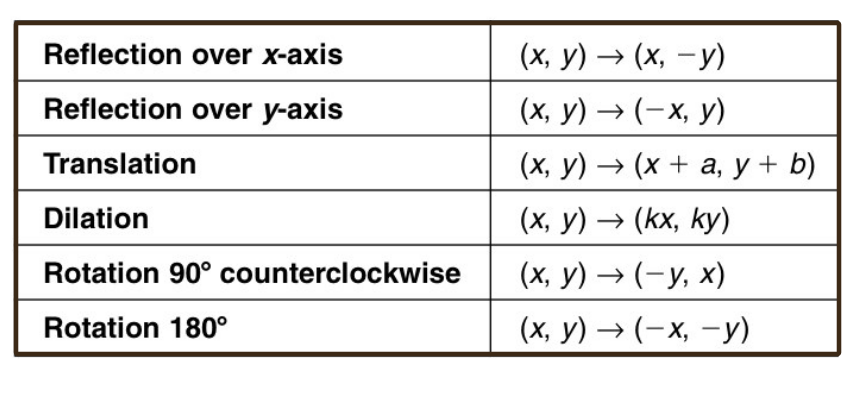
\includegraphics[width=0.8\textwidth]{transformation_r.png}
    \caption{Where common transformations send a point $(x, y)$.}
    \label{fig:transformation_r}
\end{figure}

\subsection{Order is important!}

You can combine \index{order of transformations}transformations. For
example, you can translate a function up 1, then stretch it vertically by
2.

Here is $y = 2.0 (\sin(x) + 1)$:
\begin{figure}[H]
    \centering

\begin{tikzpicture}[
tl/.style = {% tick labels
    fill=white, inner sep=1pt, font=\scriptsize,
            },                        ]
% grid
\draw[sdkblue, very thin, xstep=0.5236, ystep=0.5] (-6.6,-1.2) grid (6.6,4.2);

% y tick label
\foreach \y in {-1, -1/2, 1/2, 1, 2, 3, 4}{\node[tl,left=1mm] at (0,\y) {$\y$};}
% x tick label
\foreach \x [count=\xx from -4] in 
       {-2\pi,
        -\frac{3\pi}{2},
        -\pi,           
        -\frac{\pi}{2}, 
        { },
         \frac{\pi}{2},
         \pi, 
         \frac{3\pi}{2}, 
         2\pi
        }{\node[tl,below=1mm] at (3*0.5235*\xx,0) {$\x$};}
% axes
    \draw[->,thick] (-6.5,0) -- (6.5,0) node[right] {$x$};
    \draw[->,thick] (0,-1.25) -- (0, 4.25) node[above] {$y$};
% curve
\draw[<->,dashed,draw=black,
      domain=-6.5:6.5,samples=300,variable=\x] 
      plot (\x,{sin(deg{\x})});
\draw[<->,thick,draw=black,
      domain=-6.5:6.5,samples=300,variable=\x] 
      plot (\x,{2.0 * (sin(deg{\x}) + 1)});
\end{tikzpicture}

    \caption{A graph of the base function $\sin(x)$ and the transformed function $2(\sin(x)+1)$}
    \label{fig:translatingSin}
\end{figure}

A function is often a series of steps. Here are the steps in $f(x) = 2(\sin(x) + 1)$:
\begin{enumerate}
\item Take the sine of $x$
\item Add 1 to that
\item Multiply that by 2
\end{enumerate}
Distributing the 2 gives the same function: $f(x) = 2\sin(x) + 2$.

What if we change the order? Here are the steps in $g(x) = 2\sin(x) + 1$:
\begin{enumerate}
\item Take the sine of $x$
\item Multiply that by 2
\item Add 1 to that
\end{enumerate}
\begin{figure}[H]
    \centering

\begin{tikzpicture}[
tl/.style = {% tick labels
    fill=white, inner sep=1pt, font=\scriptsize,
            },                        ]
% grid
\draw[sdkblue, very thin, xstep=0.5236, ystep=0.5] (-6.6,-2.2) grid (6.6,4.2);

% y tick label
\foreach \y in {-2, -1, -1/2, 1/2, 1, 2, 3, 4}{\node[tl,left=1mm] at (0,\y) {$\y$};}
% x tick label
\foreach \x [count=\xx from -4] in 
       {-2\pi,
        -\frac{3\pi}{2},
        -\pi,           
        -\frac{\pi}{2}, 
        { },
         \frac{\pi}{2},
         \pi, 
         \frac{3\pi}{2}, 
         2\pi
        }{\node[tl,below=1mm] at (3*0.5235*\xx,0) {$\x$};}
% axes
    \draw[->,thick] (-6.5,0) -- (6.5,0) node[right] {$x$};
    \draw[->,thick] (0,-2.25) -- (0, 4.25) node[above] {$y$};
% curve
\draw[<->,dashed,draw=black,
      domain=-6.5:6.5,samples=300,variable=\x] 
plot (\x,{2.0 * (sin(deg{\x}) + 1)});
\draw (4, 3) node{$2(\sin(x) + 1)$};
\draw[<->,thick,draw=black,
      domain=-6.5:6.5,samples=300,variable=\x] 
      plot (\x,{2.0 * sin(deg(\x)) + 1});
\draw (2.5, -1.5) node{$2\sin(x) + 1$};
\end{tikzpicture}

    \caption{The functions $2\sin(x)+1$ in solid compared to $2(\sin(x)+1)$ in dashes.}
    \label{fig:orderMattersSin}
\end{figure}


The two curves differ by 1 everywhere. The moral: when you combine
transformations, order matters. It is socks and shoes all over again.

\begin{Exercise}[title={Transforms}, label=sine_transform]

Find a function that creates a sine wave such that the top of the first crest is
at the point $(\frac{\pi}{2}, 5)$ and the bottom of the trough that follows is at $(\pi, 1)$.


\begin{tikzpicture}[
tl/.style = {% tick labels
    fill=white, inner sep=1pt, font=\scriptsize,
            },                        ]
% grid
\draw[sdkblue, very thin, xstep=0.5236, ystep=0.5] (-1,-0.6) grid (6.6,5.2);

% y tick label
\foreach \y in {1/2, 1, 2, 3, 4, 5}{\node[tl,left=1mm] at (0,\y) {$\y$};}
% axes
    \draw[->,thick] (-0.9,0) -- (6.5,0) node[right] {$x$};
    \draw[->,thick] (0,-0.25) -- (0, 5.25) node[above] {$y$};
    % curve
    \filldraw[black] (1.570796326794897, 5)  circle(3pt) node [right, yshift=1mm]{$(\pi/2,5)$};
    \filldraw[black] (3.141592653589793, 1)  circle(3pt) node[below]{$(\pi,1)$};
    \draw[<->,thick,draw=black,
      domain=-0.5:6.5,samples=300,variable=\x] 
      plot (\x,{2.0 * sin(deg{2*\x} - 90) + 3});
\end{tikzpicture}

  
\end{Exercise}
\begin{Answer}[ref=sine_transform]

\begin{tikzpicture}[
tl/.style = {% tick labels
    fill=white, inner sep=1pt, font=\scriptsize,
            },                        ]
% grid
\draw[sdkblue, very thin, xstep=0.5236, ystep=0.5] (-1,-0.6) grid (6.6,5.2);

% y tick label
\foreach \y in {1/2, 1, 2, 3, 4, 5}{\node[tl,left=1mm] at (0,\y) {$\y$};}
% axes
    \draw[->,thick] (-0.9,0) -- (6.5,0) node[right] {$x$};
    \draw[->,thick] (0,-0.25) -- (0, 5.25) node[above] {$y$};
    % curvet
    \filldraw[black] (0.785398163397448, 3)  circle(3pt) node[right, yshift=1mm]{$(\pi/4, 3)$};
    \filldraw[black] (1.570796326794897, 5)  circle(3pt) node [right, yshift=1mm]{$(\pi/2, 5)$};
    \filldraw[black] (3.141592653589793, 1)  circle(3pt) node[below]{$(\pi, 1)$};
    \filldraw[black] (4.71238898038469, 5)  circle(3pt) node[right, yshift=1mm]{$(3\pi/2, 5)$};
    \draw[<->,thick,draw=black,
      domain=-0.5:6.5,samples=300,variable=\x] 
      plot (\x,{2.0 * sin(deg{2*\x} - 90) + 3});
    \draw[dashed,thick, draw=black] (0,3) -- (6,3);
\end{tikzpicture}

This wave has an amplitude of 2; its baseline has been translated up to 3.

This wave has wavelength of $\pi$. A sine wave usually has a
wavelength of $2\pi$, so we need to compress the $x$ axis by a factor of 2.

The crest is at $\frac{\pi}{2}$, so the wave crosses its baseline on the
way up a quarter wavelength earlier, at $\frac{\pi}{2} - \frac{\pi}{4} =
\frac{\pi}{4}$. A plain sine wave crosses its baseline on the way up at 0,
so we translate right by $\frac{\pi}{4}$: replace $x$ with
$x - \frac{\pi}{4}$.

$$f(x) = 2 \sin\left(2\left(x - \frac{\pi}{4}\right)\right) + 3 = 2\sin\left(2x - \frac{\pi}{2}\right) + 3$$

Check: $f\left(\frac{\pi}{2}\right) = 2\sin\left(\frac{\pi}{2}\right) + 3 = 5$
and $f(\pi) = 2\sin\left(\frac{3\pi}{2}\right) + 3 = 1$. Watch the
parentheses: $2\sin(2x - \frac{\pi}{4}) + 3$ shifts right by only
$\frac{\pi}{8}$.

\end{Answer}

\subsection{Effects on even and odd Functions}
Which transformations keep a function \index{symmetry}even or odd?
\begin{enumerate}
    \item Vertical shifts ($f(x) + c$) keep an \index{even function}even
          function even: $x^2 + 1$ is still a mirror image across the
          $y$-axis. They break oddness: $x^3$ is \index{odd function}odd, but
          $x^3 + 1$ is not.
    \item Horizontal shifts ($f(x - c)$) usually break both. $\sin(x)$ is
          odd, but $\sin(x - \frac{\pi}{4})$ is neither. (Careful:
          $\sin(x - \frac{\pi}{2}) = -\cos(x)$, which happens to be even.
          Always check.)
    \item Vertical stretches ($a f(x)$) and horizontal stretches ($f(bx)$)
          keep the type: $3x^2$ is even, and $(2x)^3$ is odd.
\end{enumerate}
When in doubt, compute $f(-x)$ and compare.

\begin{Exercise}[title={Inverse of a Cube}, label=inv1]
Let $f(x) = x^3$. Find $f^{-1}(8)$.
\end{Exercise}
\begin{Answer}[ref=inv1]
Solve $x^3 = 8$. Then $x = 2$, so $f^{-1}(8) = 2$.
\end{Answer}
